% !TEX root = slides.tex
%==============================================================================
\begin{frame}[t]
\label{merr7}

\frametitle{Model Error -- Likelihood construction}
\vspace*{-0.2cm}


\centerline{
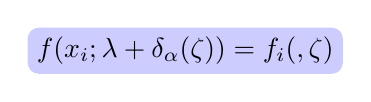
\begin{tikzpicture} \node [rounded corners,fill=blue!20] {
$f(x_i;\lambda+\delta_\alpha(\zeta))=f_i(\tlam,\zeta)$
};
\end{tikzpicture}
}

\bi
\setlength{\itemsep}{3mm}
\setlength{\itemindent}{-4.4mm}
\item Define pushed-forward means and variances

\[\mu_i(\tlam)=\EE_\zeta[f_i(\tlam,\zeta)]\qquad\quad \textrm{and}
\qquad\quad\sigma^2_i(\tlam)=\VV_\zeta[f_i(\tlam,\zeta)]\]

\item Gauss-Marginal Approximate Likelihood compares data $g_i$ and model predictions:\\
$
{\cal L}_g(\tlam) \approx \frac{1}{\left(2\pi\right)^{N/2}} \prod_{i=1}^N \frac{1}{\sigma_i(\tlam)}\exp\left(-\frac{1}{2}\left(\frac{g_i-\mu_i(\tlam)} {\sigma_i(\tlam)}\right)^2 \right)
$
\medskip
\item Non-intrusive spectral projection (NISP) with Polynomial Chaos

\centerline{
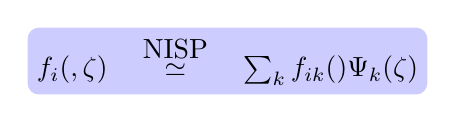
\begin{tikzpicture} \node [rounded corners,fill=blue!20] {
$f_i(\tlam,\zeta) \quad\stackrel{\textrm{NISP}}{\simeq} \quad\sum_k f_{ik}(\tlam) \Psi_k(\zeta)$
};
\end{tikzpicture}
}

\item ... provides easy access to mean and variance
\vspace*{-0.2cm}
\[\mu_i(\tlam)=f_{i0}(\tlam)\qquad\quad \textrm{and}
\qquad\quad\sigma_i^2(\tlam)=\sum_{k\neq 0} f_{ik}^2(\tlam) ||\Psi_k||^2\]

\ei

\end{frame}
%==================================================================================
